% Created by tikzDevice version 0.7.0 on 2015-04-28 20:17:12
% !TEX encoding = UTF-8 Unicode
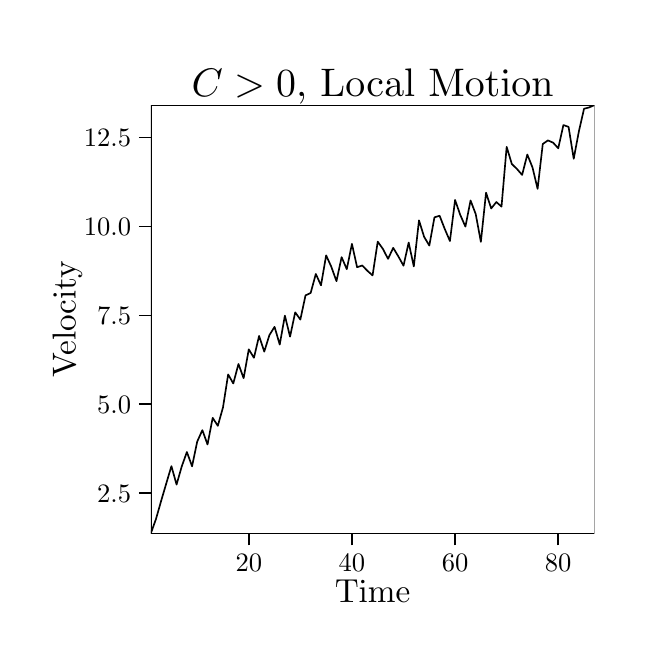
\begin{tikzpicture}[x=1pt,y=1pt]
\definecolor[named]{fillColor}{rgb}{1.00,1.00,1.00}
\path[use as bounding box,fill=fillColor,fill opacity=0.00] (0,0) rectangle (216.81,216.81);
\begin{scope}
\path[clip] (  0.00,  0.00) rectangle (216.81,216.81);
\definecolor[named]{drawColor}{rgb}{1.00,1.00,1.00}
\definecolor[named]{fillColor}{rgb}{1.00,1.00,1.00}

\path[draw=drawColor,line width= 0.6pt,line join=round,line cap=round,fill=fillColor] ( -0.00,  0.00) rectangle (216.81,216.81);
\end{scope}
\begin{scope}
\path[clip] ( 44.49, 34.03) rectangle (204.76,188.82);
\definecolor[named]{fillColor}{rgb}{1.00,1.00,1.00}

\path[fill=fillColor] ( 44.49, 34.03) rectangle (204.76,188.82);
\definecolor[named]{drawColor}{rgb}{0.00,0.00,0.00}

\path[draw=drawColor,line width= 0.6pt,line join=round] ( 44.49, 34.03) --
	( 46.35, 39.22) --
	( 48.21, 45.75) --
	( 50.08, 52.11) --
	( 51.94, 58.37) --
	( 53.80, 51.71) --
	( 55.67, 58.25) --
	( 57.53, 63.47) --
	( 59.40, 58.31) --
	( 61.26, 67.23) --
	( 63.12, 71.38) --
	( 64.99, 66.20) --
	( 66.85, 75.82) --
	( 68.71, 72.94) --
	( 70.58, 79.61) --
	( 72.44, 91.50) --
	( 74.30, 88.24) --
	( 76.17, 95.28) --
	( 78.03, 90.15) --
	( 79.90,100.58) --
	( 81.76, 97.52) --
	( 83.62,105.42) --
	( 85.49, 99.75) --
	( 87.35,105.73) --
	( 89.21,108.71) --
	( 91.08,102.29) --
	( 92.94,112.76) --
	( 94.81,105.16) --
	( 96.67,113.94) --
	( 98.53,111.34) --
	(100.40,120.07) --
	(102.26,120.95) --
	(104.12,127.82) --
	(105.99,123.71) --
	(107.85,134.53) --
	(109.72,130.40) --
	(111.58,125.21) --
	(113.44,133.88) --
	(115.31,129.54) --
	(117.17,138.68) --
	(119.03,130.26) --
	(120.90,130.88) --
	(122.76,128.95) --
	(124.63,127.30) --
	(126.49,139.49) --
	(128.35,136.88) --
	(130.22,133.27) --
	(132.08,137.25) --
	(133.94,134.16) --
	(135.81,130.80) --
	(137.67,139.16) --
	(139.53,130.53) --
	(141.40,147.17) --
	(143.26,141.21) --
	(145.13,138.09) --
	(146.99,148.27) --
	(148.85,148.85) --
	(150.72,144.04) --
	(152.58,139.70) --
	(154.44,154.55) --
	(156.31,149.16) --
	(158.17,144.93) --
	(160.04,154.35) --
	(161.90,149.45) --
	(163.76,139.41) --
	(165.63,157.18) --
	(167.49,151.48) --
	(169.35,153.80) --
	(171.22,152.15) --
	(173.08,173.74) --
	(174.95,167.54) --
	(176.81,165.74) --
	(178.67,163.60) --
	(180.54,170.96) --
	(182.40,166.36) --
	(184.26,158.57) --
	(186.13,174.77) --
	(187.99,176.07) --
	(189.86,175.26) --
	(191.72,173.23) --
	(193.58,181.62) --
	(195.45,180.96) --
	(197.31,169.44) --
	(199.17,179.31) --
	(201.04,187.50) --
	(202.90,188.00) --
	(204.76,188.82);

\path[draw=drawColor,line width= 0.6pt,line join=round,line cap=round] ( 44.49, 34.03) rectangle (204.76,188.82);
\end{scope}
\begin{scope}
\path[clip] (  0.00,  0.00) rectangle (216.81,216.81);
\definecolor[named]{drawColor}{rgb}{0.00,0.00,0.00}

\node[text=drawColor,anchor=base east,inner sep=0pt, outer sep=0pt, scale=  0.96] at ( 37.37, 45.33) {2.5};

\node[text=drawColor,anchor=base east,inner sep=0pt, outer sep=0pt, scale=  0.96] at ( 37.37, 77.44) {5.0};

\node[text=drawColor,anchor=base east,inner sep=0pt, outer sep=0pt, scale=  0.96] at ( 37.37,109.56) {7.5};

\node[text=drawColor,anchor=base east,inner sep=0pt, outer sep=0pt, scale=  0.96] at ( 37.37,141.67) {10.0};

\node[text=drawColor,anchor=base east,inner sep=0pt, outer sep=0pt, scale=  0.96] at ( 37.37,173.79) {12.5};
\end{scope}
\begin{scope}
\path[clip] (  0.00,  0.00) rectangle (216.81,216.81);
\definecolor[named]{drawColor}{rgb}{0.00,0.00,0.00}

\path[draw=drawColor,line width= 0.6pt,line join=round] ( 40.22, 48.63) --
	( 44.49, 48.63);

\path[draw=drawColor,line width= 0.6pt,line join=round] ( 40.22, 80.75) --
	( 44.49, 80.75);

\path[draw=drawColor,line width= 0.6pt,line join=round] ( 40.22,112.86) --
	( 44.49,112.86);

\path[draw=drawColor,line width= 0.6pt,line join=round] ( 40.22,144.98) --
	( 44.49,144.98);

\path[draw=drawColor,line width= 0.6pt,line join=round] ( 40.22,177.09) --
	( 44.49,177.09);
\end{scope}
\begin{scope}
\path[clip] (  0.00,  0.00) rectangle (216.81,216.81);
\definecolor[named]{drawColor}{rgb}{0.00,0.00,0.00}

\path[draw=drawColor,line width= 0.6pt,line join=round] ( 79.90, 29.77) --
	( 79.90, 34.03);

\path[draw=drawColor,line width= 0.6pt,line join=round] (117.17, 29.77) --
	(117.17, 34.03);

\path[draw=drawColor,line width= 0.6pt,line join=round] (154.44, 29.77) --
	(154.44, 34.03);

\path[draw=drawColor,line width= 0.6pt,line join=round] (191.72, 29.77) --
	(191.72, 34.03);
\end{scope}
\begin{scope}
\path[clip] (  0.00,  0.00) rectangle (216.81,216.81);
\definecolor[named]{drawColor}{rgb}{0.00,0.00,0.00}

\node[text=drawColor,anchor=base,inner sep=0pt, outer sep=0pt, scale=  0.96] at ( 79.90, 20.31) {20};

\node[text=drawColor,anchor=base,inner sep=0pt, outer sep=0pt, scale=  0.96] at (117.17, 20.31) {40};

\node[text=drawColor,anchor=base,inner sep=0pt, outer sep=0pt, scale=  0.96] at (154.44, 20.31) {60};

\node[text=drawColor,anchor=base,inner sep=0pt, outer sep=0pt, scale=  0.96] at (191.72, 20.31) {80};
\end{scope}
\begin{scope}
\path[clip] (  0.00,  0.00) rectangle (216.81,216.81);
\definecolor[named]{drawColor}{rgb}{0.00,0.00,0.00}

\node[text=drawColor,anchor=base,inner sep=0pt, outer sep=0pt, scale=  1.20] at (124.63,  9.03) {Time};
\end{scope}
\begin{scope}
\path[clip] (  0.00,  0.00) rectangle (216.81,216.81);
\definecolor[named]{drawColor}{rgb}{0.00,0.00,0.00}

\node[text=drawColor,rotate= 90.00,anchor=base,inner sep=0pt, outer sep=0pt, scale=  1.20] at ( 17.30,111.43) {Velocity};
\end{scope}
\begin{scope}
\path[clip] (  0.00,  0.00) rectangle (216.81,216.81);
\definecolor[named]{drawColor}{rgb}{0.00,0.00,0.00}

\node[text=drawColor,anchor=base,inner sep=0pt, outer sep=0pt, scale=  1.44] at (124.63,191.84) {$C > 0$, Local Motion};
\end{scope}
\end{tikzpicture}
